\documentclass{standalone}
\usepackage[utf8]{inputenc}
\usepackage{tikz}
\usetikzlibrary{shapes.geometric, arrows,calc,positioning}

\tikzstyle{rawdata} = [rectangle, rounded corners, minimum width=3cm, minimum height=1cm,text centered, draw=black, fill=red!30]

\tikzstyle{analysisdata} = [rectangle, rounded corners, minimum width=3cm, minimum height=1cm,text centered, draw=black, fill=green!30]

\tikzstyle{csv} = [rectangle, minimum width=3cm, minimum height=1cm, text centered, text width=5cm, draw=black, fill=purple!30]

\tikzstyle{io} = [trapezium, trapezium left angle=90, trapezium right angle=110, minimum height=1cm, text centered, draw=black, fill=blue!30]
\tikzstyle{process} = [rectangle, minimum width=3cm, minimum height=1cm, text centered, text width=3cm, draw=black, fill=orange!30]
\tikzstyle{decision} = [diamond, minimum width=3cm, minimum height=1cm, text centered, draw=black, fill=green!30]
\tikzstyle{arrow} = [thick,->,>=stealth]

\begin{document}

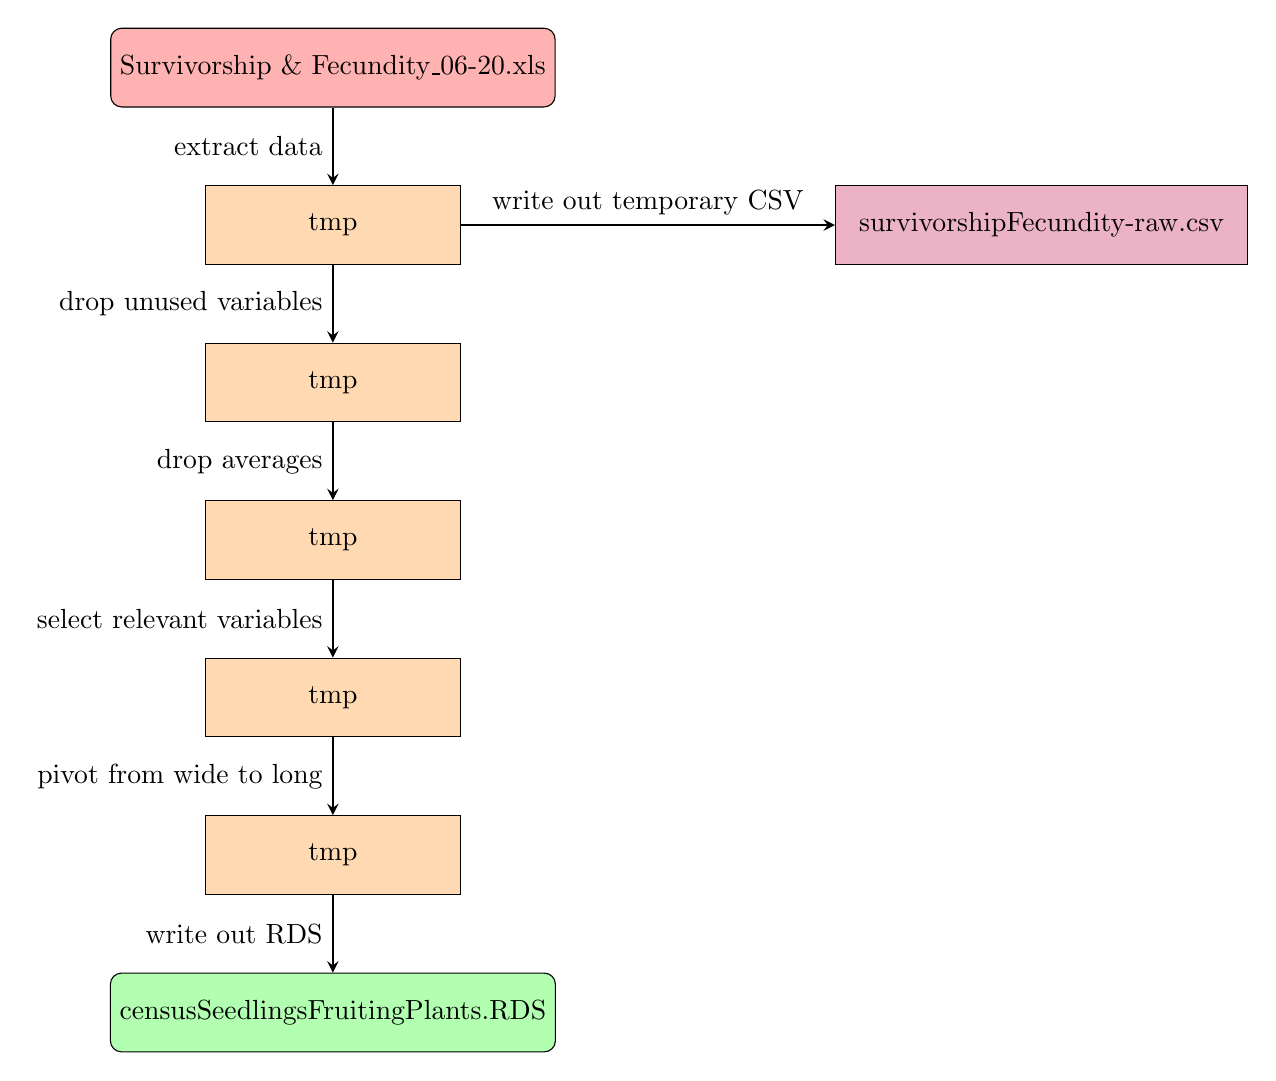
\begin{tikzpicture}[node distance=2cm]

\node (start) [rawdata] {Survivorship \& Fecundity\_06-20.xls};
\node (tmp1) [process, below of=start] {tmp};
\node (tmp2) [process, below of=tmp1] {tmp};
\node (csv1) [csv, right of=tmp1, xshift=7cm] {survivorshipFecundity-raw.csv};
\node (tmp3) [process, below of=tmp2] {tmp};
\node (tmp4) [process, below of=tmp3] {tmp};
\node (tmp5) [process, below of=tmp4] {tmp};
\node (stop) [analysisdata, below of=tmp5] {censusSeedlingsFruitingPlants.RDS};

\draw [arrow] (start) -- node[anchor=east] {extract data} (tmp1);
\draw [arrow] (tmp1) -- node[anchor=south] {write out temporary CSV} (csv1);
\draw [arrow] (tmp1) -- node[anchor=east] {drop unused variables} (tmp2);
\draw [arrow] (tmp2) -- node[anchor=east] {drop averages} (tmp3);
\draw [arrow] (tmp3) -- node[anchor=east] {select relevant variables} (tmp4);
\draw [arrow] (tmp4) -- node[anchor=east] {pivot from wide to long} (tmp5);
\draw [arrow] (tmp5) -- node[anchor=east] {write out RDS} (stop);

\end{tikzpicture}

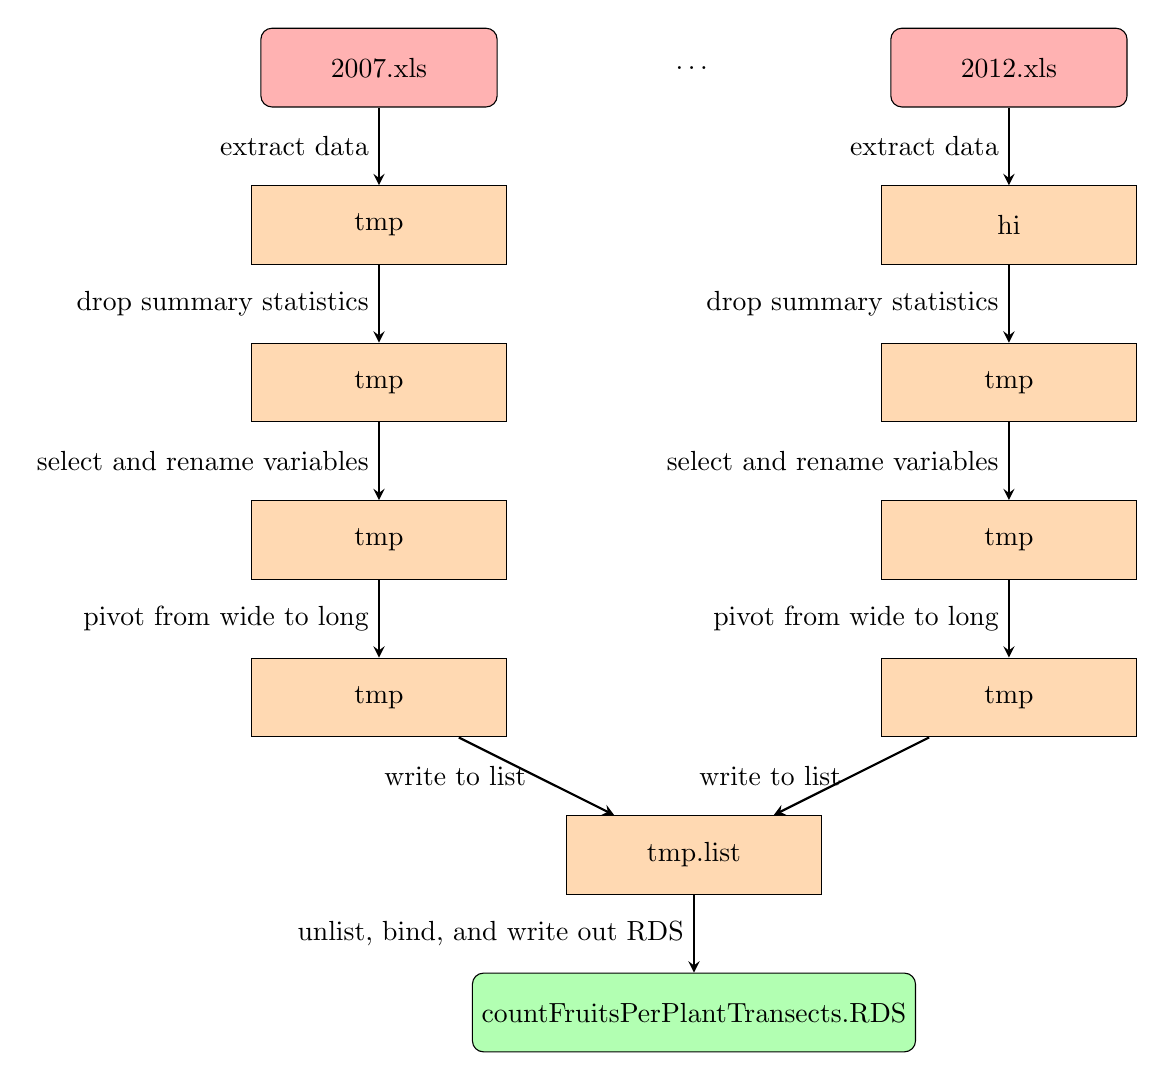
\begin{tikzpicture}[node distance=2cm]

\node (start) [rawdata] {2007.xls};
\node (start2) [rawdata, right of=start,xshift=6cm] {2012.xls};
    \node (years) at ($(start)!.5!(start2)$) {\ldots};
\node (tmp1) [process, below of=start] {tmp};
\node (tmp2) [process, below of=tmp1] {tmp};
\node (tmp3) [process, below of=tmp2] {tmp};
\node (tmp4) [process, below of=tmp3] {tmp};
\node (tmp5) [process, below of=tmp4,fill=white,white] {};
%
\node (tmp12) [process, below of=start2] {hi};
\node (tmp22) [process, below of=tmp12] {tmp};
\node (tmp32) [process, below of=tmp22] {tmp};
\node (tmp42) [process, below of=tmp32] {tmp};
\node (tmp52) [process, below of=tmp42,fill=white,white] {};
%
\node (list) [process, right of=tmp5,xshift=2cm] {tmp.list};
\node (stop) [analysisdata, below of=list] {countFruitsPerPlantTransects.RDS};

\draw [arrow] (start) -- node[anchor=east] {extract data} (tmp1);
\draw [arrow] (tmp1) -- node[anchor=east] {drop summary statistics} (tmp2);
\draw [arrow] (tmp2) -- node[anchor=east] {select and rename variables} (tmp3);
\draw [arrow] (tmp3) -- node[anchor=east] {pivot from wide to long} (tmp4);
\draw [arrow] (tmp4) -- node[anchor=east] {write to list} (list);
\draw [arrow] (start2) -- node[anchor=east] {extract data} (tmp12);
\draw [arrow] (tmp12) -- node[anchor=east] {drop summary statistics} (tmp22);
\draw [arrow] (tmp22) -- node[anchor=east] {select and rename variables} (tmp32);
\draw [arrow] (tmp32) -- node[anchor=east] {pivot from wide to long} (tmp42);
\draw [arrow] (tmp42) -- node[anchor=east] {write to list} (list);
%
\draw [arrow] (list) -- node[anchor=east] {unlist, bind, and write out RDS} (stop);

\end{tikzpicture}

% damaged and undamaged 2013-2018
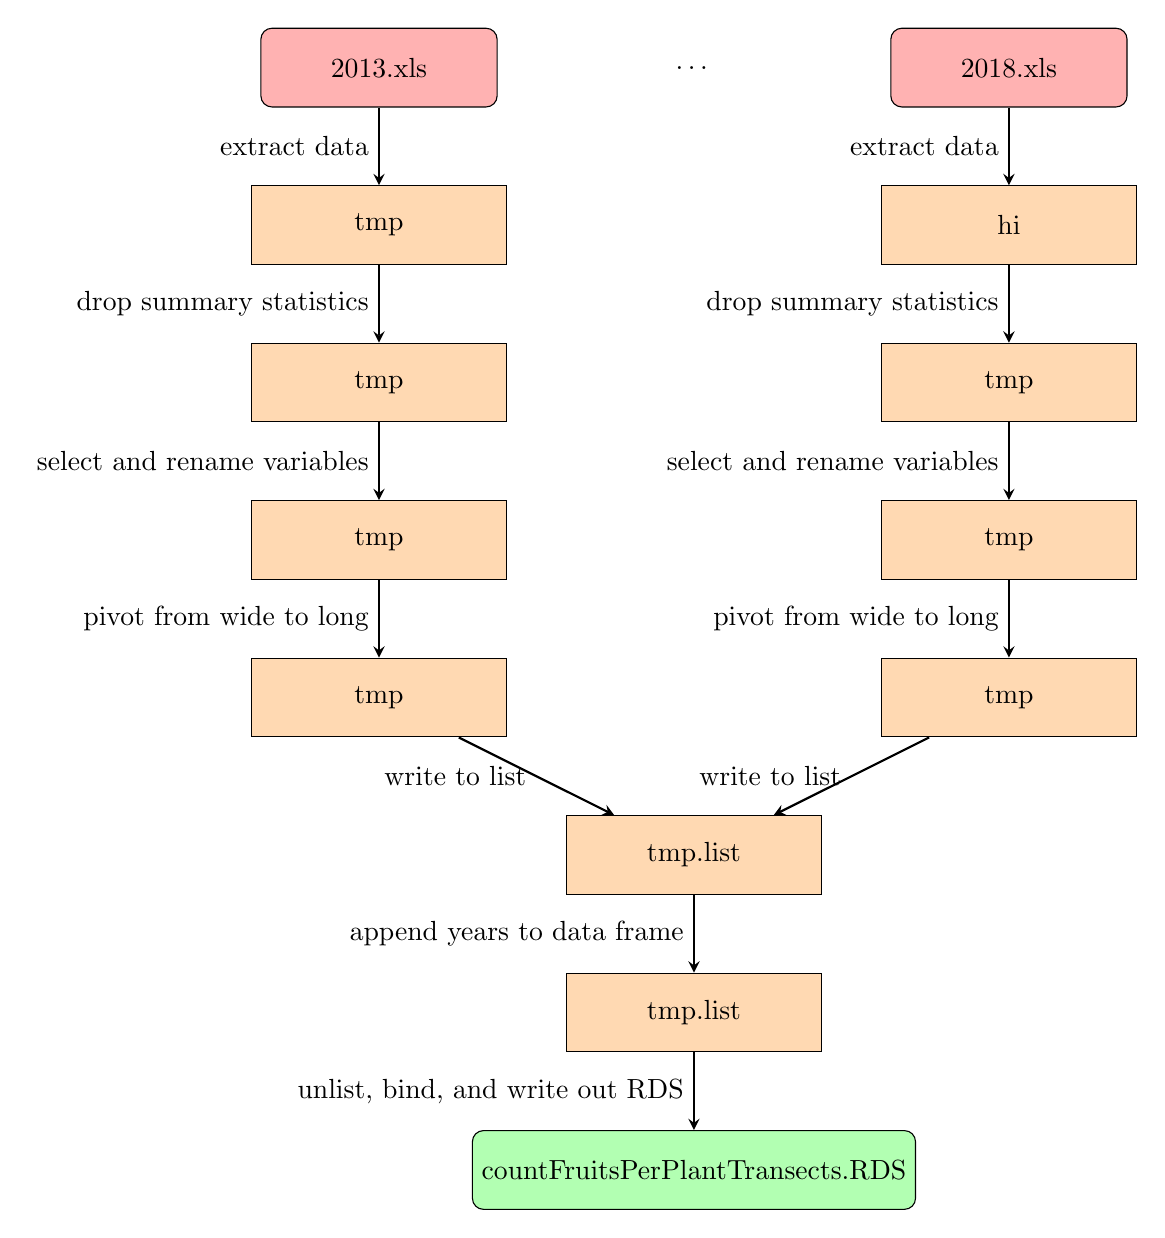
\begin{tikzpicture}[node distance=2cm]

\node (start) [rawdata] {2013.xls};
\node (start2) [rawdata, right of=start,xshift=6cm] {2018.xls};
    \node (years) at ($(start)!.5!(start2)$) {\ldots};
\node (tmp1) [process, below of=start] {tmp};
\node (tmp2) [process, below of=tmp1] {tmp};
\node (tmp3) [process, below of=tmp2] {tmp};
\node (tmp4) [process, below of=tmp3] {tmp};
\node (tmp5) [process, below of=tmp4,fill=white,white] {};
%
\node (tmp12) [process, below of=start2] {hi};
\node (tmp22) [process, below of=tmp12] {tmp};
\node (tmp32) [process, below of=tmp22] {tmp};
\node (tmp42) [process, below of=tmp32] {tmp};
\node (tmp52) [process, below of=tmp42,fill=white,white] {};
%
\node (list) [process, right of=tmp5,xshift=2cm] {tmp.list};
\node (list2) [process, below of=list] {tmp.list};
\node (stop) [analysisdata, below of=list2] {countFruitsPerPlantTransects.RDS};

\draw [arrow] (start) -- node[anchor=east] {extract data} (tmp1);
\draw [arrow] (tmp1) -- node[anchor=east] {drop summary statistics} (tmp2);
\draw [arrow] (tmp2) -- node[anchor=east] {select and rename variables} (tmp3);
\draw [arrow] (tmp3) -- node[anchor=east] {pivot from wide to long} (tmp4);
\draw [arrow] (tmp4) -- node[anchor=east] {write to list} (list);
\draw [arrow] (start2) -- node[anchor=east] {extract data} (tmp12);
\draw [arrow] (tmp12) -- node[anchor=east] {drop summary statistics} (tmp22);
\draw [arrow] (tmp22) -- node[anchor=east] {select and rename variables} (tmp32);
\draw [arrow] (tmp32) -- node[anchor=east] {pivot from wide to long} (tmp42);
\draw [arrow] (tmp42) -- node[anchor=east] {write to list} (list);
\draw [arrow] (list) -- node[anchor=east] {append years to data frame} (list2);
\draw [arrow] (list2) -- node[anchor=east] {unlist, bind, and write out RDS} (stop);

\end{tikzpicture}


\end{document}